\chapter{Metodologia}\label{ch:method}

O método é uma avaliação de terras multicritério na tradição da avaliação de terras da
FAO (Food and Agriculture Organization), hoje operacionalizada no \emph{Global Agro-Ecological
Zones} (GAEZ~v4) \citep{noauthor_global_2021,sys_land_1991}. Ele é implementado
nativamente na plataforma de observação da Terra, estendido com um zoneamento não supervisionado e
uma projeção CMIP6, e concebido para validação contra o uso atual da terra. O trabalho corre em duas
fases. A \textbf{Fase~A} constrói o atlas de potencial biofísico e a projeção climática apenas a
partir do catálogo público. A \textbf{Fase~B} integra o uso atual da terra, as unidades municipais e
um indicador independente de produtividade para o mascaramento, a análise potencial \emph{versus}
realizado e a validação. A Figura~\ref{fig:metodologia} resume esse fluxo, do catálogo público ao
atlas de viabilidade final.

\begin{figure}[H]
\centering
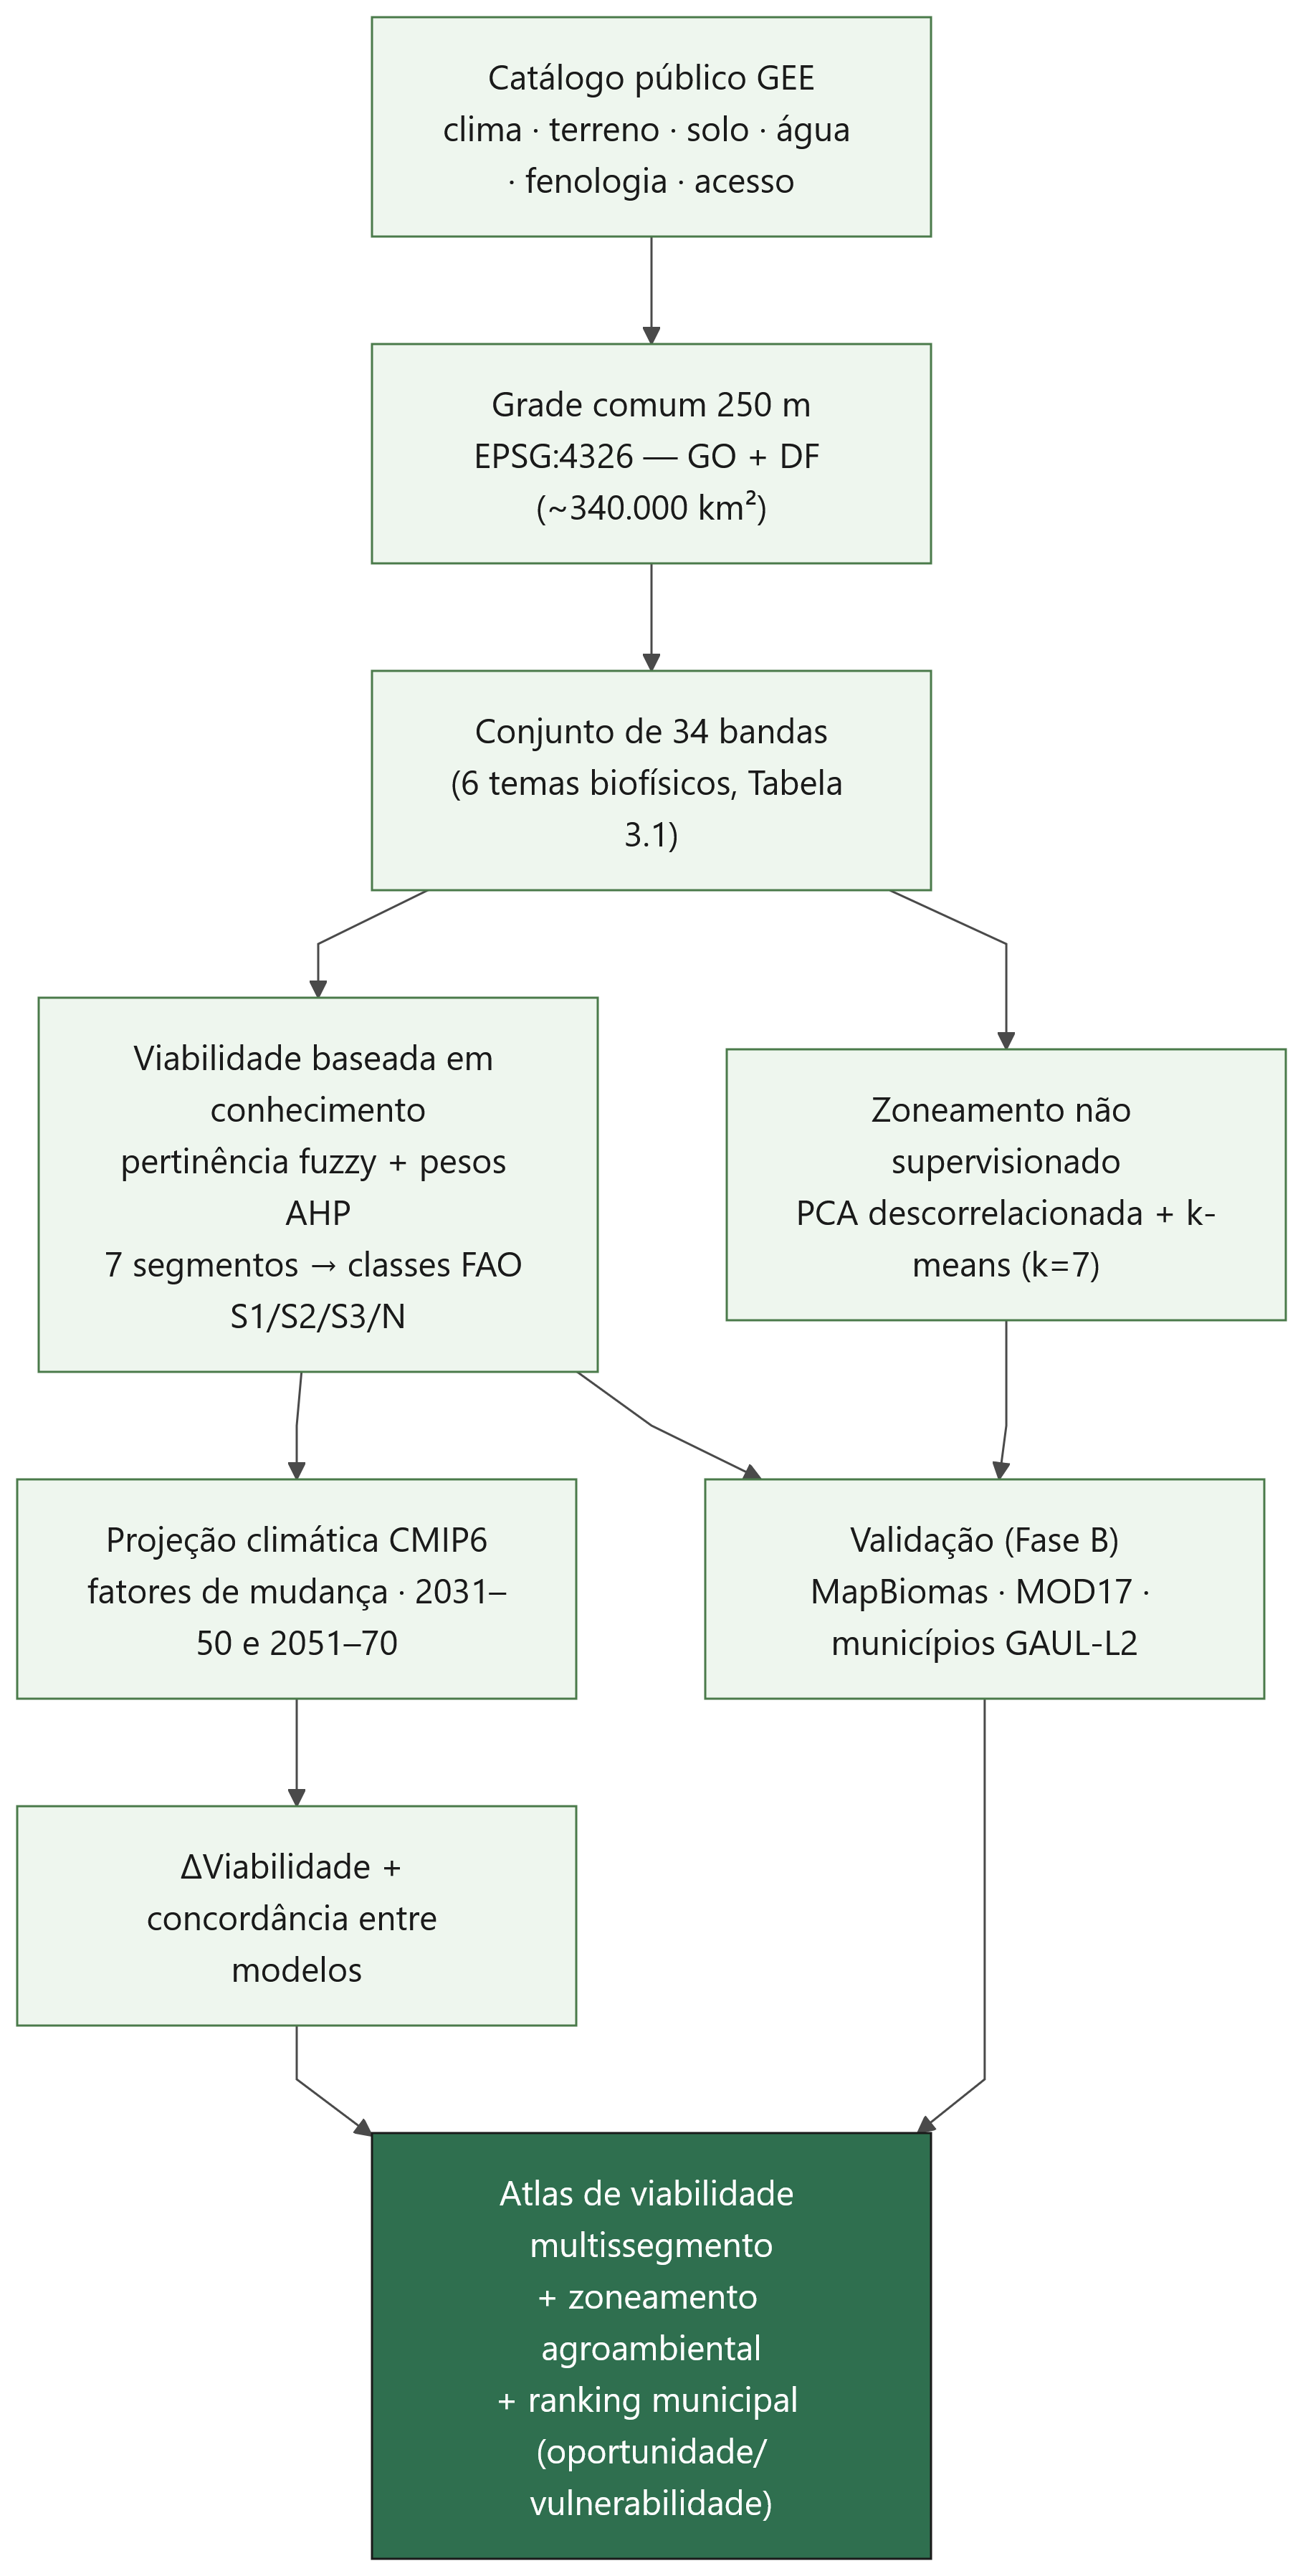
\includegraphics[width=0.75\textwidth]{Chapters/Figures/diagrama_metodologia.png}
\caption{Visão geral do fluxo metodológico, do catálogo público do Google Earth Engine ao atlas de viabilidade multissegmento, ao zoneamento agroambiental e ao ranking municipal.}\label{fig:metodologia}
\end{figure}

\section{Engenharia de atributos --- o conjunto de 34 bandas}\label{sec:feature-eng}

Todas as entradas são harmonizadas para uma grade comum de 250~m no sistema EPSG:4326. Os campos
climáticos de resolução grossa são reamostrados bilinearmente, enquanto os rasters finos de solo e
terreno são agregados por média espacial. Seis temas contínuos são concatenados em um único conjunto
de 34 bandas (Tabela~\ref{tab:stack}). É produzida também uma cópia padronizada do conjunto, em que cada banda $b$ recebe um escore~z com a
média territorial $\mu_b$ e o desvio padrão $\sigma_b$:
\begin{equation*}
  z_b(x) = \frac{x_b - \mu_b}{\sigma_b}.
\end{equation*}
Essa padronização serve ao agrupamento, para que variáveis de unidades díspares contribuam de forma
comparável para a distância euclidiana.

Um sétimo tema --- a cobertura genérica da terra --- é construído como camada de máscara e de
contexto e é deliberadamente excluído do conjunto. As fórmulas de derivação por variável
(agregação climática; graus-dia de crescimento pelo Método~1 de \citet[p.~292]{mcmaster_growing_1997},
aqui aplicado a médias mensais; índice de umidade topográfica \citep[p.~48, eq.~8]{beven_physically_1979};
regressão harmônica da fenologia, na linha de aplicações a savanas \citep[p.~96]{levine_time_2019},
estendida com um termo semianual) estão no Anexo~\ref{anx:derivations}; os temas
são resumidos abaixo.

\begin{table}[H]
\centering
\caption{Composição do conjunto de 34 bandas.}\label{tab:stack}
\begin{tabular}{@{}lp{10cm}r@{}}
\toprule
Tema & Variáveis & Contagem \\
\midrule
Clima & Precipitação anual; evapotranspiração potencial anual, evapotranspiração real e déficit
  hídrico climático; sazonalidade da precipitação; duração da estação seca; precipitação da estação
  chuvosa; índice de aridez; umidade do solo; déficit de pressão de vapor; radiação solar; graus-dia
  de crescimento; temperatura média do trimestre mais quente e do mais frio & 14 \\
Terreno & Elevação; declive; componente norte da orientação; componente leste da orientação; índice
  de posição topográfica; índice de umidade topográfica & 6 \\
Solo (0--30~cm) & Argila; areia; carbono orgânico; pH (H$_2$O); densidade aparente; 
  teor de água disponível para as plantas & 6 \\
Água & Distância para água permanente; sazonalidade da água de superfície; densidade de drenagem & 3 \\
Fenologia & NDVI médio; amplitude sazonal; mês de pico; integral anual & 4 \\
Acessibilidade & Logaritmo do tempo de viagem à cidade mais próxima & 1 \\
\midrule
\textbf{Total} & & \textbf{34} \\
\bottomrule
\end{tabular}
\end{table}

As variáveis climáticas derivam de uma climatologia mensal de 1991--2020 por uma transformação
determinística reutilizada sem alteração para o clima futuro do CMIP6 (\S\ref{sec:cmip6}). É essa
identidade dos caminhos de derivação que torna a mudança projetada um sinal puramente climático.

O terreno vem de um modelo digital de elevação (MDE) de 30~m (com a orientação decomposta em
componentes norte e leste). O solo é a média das profundidades de 0, 10 e 30~cm de seis
propriedades das camadas OpenLandMap v0.2 a 250~m. % TODO(Zotero): citar Hengl (2018), OpenLandMap SOL v02
A água combina a distância à água permanente, definida como ocorrência superior a 80\% no JRC Global
Surface Water \citep{pekel_high-resolution_2016}, a sazonalidade da água de superfície (número de meses
com água no ano) do mesmo produto e a densidade de drenagem derivada da acumulação de fluxo do
HydroSHEDS (uma fração de células de canal, com faixa empírica $\approx$~0--0,15, que governa seus
limiares de pertinência). A fenologia é composta
por quatro parâmetros harmônicos do ciclo sazonal de NDVI. A acessibilidade é o logaritmo do tempo
de viagem até a cidade mais próxima.

A cobertura genérica da terra gera as máscaras de áreas \emph{excluídas} e \emph{disponíveis}, além
de frações de cobertura por classe para contexto. Essa camada é derivada do MapBiomas (coleção~10)
para melhor refletir a realidade brasileira. 
Na Fase~B, o mesmo MapBiomas alimenta,
por uma derivação distinta (papel de uso realizado por cultura, não um agrupamento genérico de
cobertura), o sinal de uso atual da terra.

\section{Viabilidade baseada em conhecimento (pertinência fuzzy + AHP)}\label{sec:suitability}

Para cada segmento, a viabilidade é um agregado ponderado de pertinências fuzzy dos fatores. Ela é
mascarada pela cobertura da terra e classificada nas classes da FAO, seguindo a extensão fuzzy/AHP
do arcabouço de avaliação de terras da FAO \citep{nisar_ahamed_gis-based_2000,yaghmaeian_mahabadi_land_2012}. A
especificação completa por segmento --- fator, peso, forma e limiares --- está na Tabela~\ref{tab:spec-longtable} do Anexo.

Os limiares móveis (não fixados por um padrão técnico, como um limite legal de declive) foram
ancorados empiricamente antes de fixados: para cada fator candidato, a distribuição percentílica
($P_5 \text{~e~} P_{95}$) foi extraída sobre a terra \emph{disponível} da AOI e, separadamente, sobre os
pixels realizados de cada segmento no MapBiomas, e o limiar teórico obtido da literatura só foi mantido quando 
coerente com essa distribuição amostral --- caso contrário, deslocado para dentro do intervalo realmente observado 
em GO~e~DF, sem abandonar a forma funcional nem a ordenação relativa.

\subsection{Padronização da pertinência fuzzy}\label{sec:fuzzy-standard}

O valor $x$ de cada fator é mapeado para uma pertinência $\mu(x) \in [0,1]$ por uma função linear por
partes --- simplificação linear das funções de pertinência contínuas usadas em avaliação fuzzy de
terras, como o modelo sigmoidal \emph{Semantic Import} \citep[pp.~80--83]{yaghmaeian_mahabadi_land_2012}
---, de uma entre três formas. A forma \textbf{crescente} (limiar inferior
$a$, superior $b$) é
\begin{equation*}
  \mu(x) = \mathrm{clamp}\!\left(\frac{x-a}{b-a},\, 0,\, 1\right);
\end{equation*}
a forma \textbf{decrescente} é o seu complemento $\mathrm{clamp}((b-x)/(b-a),\, 0,\, 1)$; e a forma
\textbf{intervalar} (trapezoidal), com $a < b \le c < d$, cresce de $a$ a $b$, satura em 1 no
intervalo ótimo $[b,c]$ e decresce de $c$ a $d$:
\begin{equation*}
  \mu(x) = \mathrm{clamp}\!\left(\min\!\left(\frac{x-a}{b-a},\; 1,\; \frac{d-x}{d-c}\right),\, 0,\, 1\right).
\end{equation*}

\subsection{Agregação, mascaramento e classificação}\label{sec:aggregation}

Os seis segmentos de produção e energia combinam suas pertinências por uma \textbf{média geométrica
ponderada}. Com pesos $w_i \ge 0$ normalizados de modo que $\sum_i w_i = 1$,
\begin{equation*}
  S = \exp\!\left(\sum_{i=1}^{n} w_i \ln\!\big(\max(\mu_i,\,\varepsilon)\big)\right),
   \qquad \varepsilon = 10^{-3}.
\end{equation*}

A média geométrica impõe o comportamento de \textbf{fator limitante}: uma única pertinência próxima
de zero deprime fortemente o agregado --- o que é agronomicamente correto, já que um bom solo não
compensa a ausência de chuva. O piso $\varepsilon$ mantém um fator plenamente limitante como uma
penalidade forte, porém finita, em vez de $\ln(0)$; a exclusão dura é delegada ao mascaramento.

\textbf{A conservação é a exceção}: por ser um índice de valor/prioridade, e não uma viabilidade de
crescimento, ela é agregada pela \textbf{média aritmética ponderada} compensatória
$S = \sum_i w_i \mu_i$. O valor de conservação decorre da força em \emph{qualquer um} de vários
critérios parcialmente substituíveis entre si --- conectividade, heterogeneidade de habitat, serviço
de carbono, serviço de água --- de modo que uma pontuação baixa em um deles não deve vetar os demais.

A viabilidade contínua $S$ é então classificada nas quatro classes da FAO nos limiares $0{,}25$,
$0{,}50$ e $0{,}75$:
\begin{equation*}
  \text{class}(S) = \begin{cases}
   \mathrm{N}  & S < 0{,}25 \\
   \mathrm{S3} & 0{,}25 \le S < 0{,}50 \\
   \mathrm{S2} & 0{,}50 \le S < 0{,}75 \\
   \mathrm{S1} & S \ge 0{,}75,
\end{cases}
\end{equation*}
onde $\mathrm{N}$ é \emph{não viável} e $\mathrm{S3}$, $\mathrm{S2}$, $\mathrm{S1}$ são,
respectivamente, \emph{marginalmente}, \emph{moderadamente} e \emph{altamente viável}.

\subsection{Ponderação AHP e sensibilidade dos pesos}\label{sec:ahp}

Os pesos dos fatores são prioridades do Processo Analítico Hierárquico (AHP) \citep{saaty_analytic_1987}.
Para um segmento com $n$ fatores, elicita-se uma matriz Saaty de comparação par a par
$A = [a_{ij}]$ (escala 1--9, $a_{ji} = 1/a_{ij}$). O vetor de prioridades $w$ aproxima o seu autovetor
principal normalizado pela média das linhas da matriz de colunas normalizadas, e $\lambda_{\max}$ é
estimado pela média de $(Aw)_i / w_i$ \citep[pp.~4--5, eq.~1]{frish_enhancing_2025}. A coerência interna da
elicitação é quantificada pela razão de consistência \citep[p.~171]{saaty_analytic_1987}:
\begin{equation*}
  \mathrm{RC} = \frac{\mathrm{IC}}{\mathrm{RI}}, \qquad
   \mathrm{IC} = \frac{\lambda_{\max} - n}{n - 1},
\end{equation*}
onde $\lambda_{\max}$ é o autovalor principal (estimado como acima) e $\mathrm{RI}$ é o valor esperado do índice aleatório
para a ordem $n$. Uma ponderação é aceita quando $\mathrm{RC} \le 0{,}10$. Cada matriz de comparação
par a par é registrada por completo. Todos os segmentos são folgadamente consistentes: $0{,}0015$ é a
maior razão de consistência entre os sete (Tabela~\ref{tab:ahp-cr} do Anexo). Os pesos se apoiam,
assim, em uma elicitação auditável e internamente coerente, e não em mera afirmação.

Os próprios pesos, além dos limiares, foram revistos frente à distribuição amostral: para cada fator, 
a amplitude interquartil ($P_{75}-P_{25}$) sobre a terra disponível é comparada à amplitude do seu próprio limiar de pertinência. Um
fator cuja distribuição real é estreita frente a esse intervalo é, na prática, quase constante em
GO~e~DF --- toda a área recebe uma pertinência próxima de 1, e o fator não separa uma célula da
outra --- por mais importante que a literatura o considere \emph{a priori}. A revisão desloca peso
dos fatores de baixo poder discriminante para os de alto poder discriminante dentro do mesmo
segmento, renormalizando para somar~1; a literatura fixa a \emph{forma} funcional de cada
pertinência e o conjunto de fatores candidatos, mas não mais congela a ordem final de importância
quando a evidência amostral aponta o contrário. A matriz
de comparação par a par (Tabela~\ref{tab:ahp-cr} do Anexo) é reconstruída a partir dos novos pesos,
preservando a razão de consistência $\le 0{,}10$.

Como os pesos são subjetivos, sua influência é adicionalmente limitada por uma perturbação de
$\pm 20\%$, um peso de cada vez: cada peso é ampliado e reduzido em 20\% (com renormalização), e a
amplitude $S_{\max} - S_{\min}$ da viabilidade resultante é relatada como banda de robustez por
segmento, sendo esta a medida de incerteza de cada superfície do presente.

\section{Zoneamento não supervisionado}\label{sec:zoning}

GO~e~DF são particionados em zonas agroambientais por agrupamento k-means sobre uma representação
\textbf{descorrelacionada} do conjunto padronizado. Agrupar as 34 bandas brutas resolve apenas três
zonas de baixa expressividade: o território é climaticamente quase uniforme, e as quatorze bandas
climáticas colineares dominam a geometria euclidiana e puxam a partição para o gradiente climático
fraco. Três passos descorrelacionam a entrada antes do agrupamento:

\begin{enumerate}
  \item do conjunto padronizado de 34 bandas é obtido um subconjunto curado de 15 bandas
    (descartando bandas colineares ou quase constantes);
  \item no subconjunto curado é feita uma ponderação por bloco temático;
  \item o subconjunto ponderado alimenta uma PCA (retendo $\geq$~90\% da variância); 
  \item a PCA é utilizado num particionamento k-means fora da plataforma (silhueta $+$ Davies--Bouldin $+$ \emph{gap} $\rightarrow k$);
  \item do particionamento é feita uma classificação pelo centroide mais próximo no espaço de componentes principais;
  \item esta classificação tem como resultado o mapa de zonas agroambientais.
\end{enumerate}

O \textbf{subconjunto curado de 15 bandas} remove bandas quase duplicadas --- mantendo a aridez em vez
do par precipitação/evapotranspiração, um índice térmico, e a argila em vez do par
areia/densidade aparente --- além das bandas quase constantes. A \textbf{ponderação por bloco temático}
divide cada banda pela raiz quadrada do número de bandas no seu tema, para que a influência de um tema não escale
com o número de bandas. E a \textbf{PCA} rotaciona o subconjunto ponderado para seus eixos principais,
retendo o menor número de componentes que expliquem $\geq$~90\% da variância.

Os componentes principais são a solução contínua (relaxada) dos indicadores de pertença do k-means,
de modo que agrupar no subespaço dos primeiros componentes aproxima a partição k-means do espaço
original; essa é a base teórica para agrupar no espaço de componentes principais em vez de sobre o
conjunto bruto \citep[Teor.~3.1]{ding_k-means_2004}. O k-means, ajustado nesse espaço, busca a partição que minimiza a soma intragrupo
dos quadrados das distâncias aos centroides $c_k$:
\begin{equation*}
  \min_{\{C_k\}} \sum_{k=1}^{K} \sum_{x \in C_k} \lVert x - c_k \rVert^2.
\end{equation*}

O número de zonas é examinado em $k = 2,\dots,20$ pela silhueta média
\citep[p.~59]{rousseeuw_silhouettes_1987}, pelo índice de Davies--Bouldin \citep{davies_cluster_1979},
pela estatística de \emph{gap} % TODO(Zotero): citar Tibshirani, Walther & Hastie (2001) quando o PDF estiver no Zotero
e pela estabilidade de subamostras (índice de Rand ajustado, ARI, em \emph{bootstrap}); uma revisão
desses índices está em \citet{ikotun_cluster_2025}. Neste território fracamente agrupado nenhum
índice decide sozinho. A silhueta é quase plana (0,161--0,187), com máximo em $k=10$ ($0{,}187$).
O Davies--Bouldin é alto para $k \le 6$ (1,65--1,87) e praticamente plano de $k=7$ a $20$
(1,50--1,57, mínimo de 1,504 em $k=19$), sem discriminar nessa faixa. O \emph{gap} cresce quase
monotonicamente e, pelo critério do primeiro $k$ com $\mathrm{gap}(k) \geq \mathrm{gap}(k+1) - s_{k+1}$,
só se estabiliza em $k=14$: indica que o território comporta mais de dez agrupamentos, mas não
aponta um $k$ abaixo disso. O argumento decisivo é a estabilidade. Na faixa $k \geq 7$, em que o
Davies--Bouldin deixa de penalizar a partição, só $k=9$ (ARI $=0{,}970$) e $k=10$ (ARI $=0{,}962$)
são estáveis sob subamostragem; os demais ficam entre $0{,}676$ e $0{,}887$. As partições grossas
$k=2$, $3$ e $5$ também são estáveis (ARI $0{,}96$--$0{,}98$), mas têm Davies--Bouldin bem pior e
zonas agregadas demais para distinguir sete segmentos. Adota-se $k = 10$, que combina a silhueta
mais alta do intervalo com uma estabilidade equivalente à de $k=9$ (a diferença de ARI é menor que
o seu desvio-padrão entre réplicas, 0,011--0,016).

\textbf{Estimação.} O agrupamento é estimado fora da plataforma sobre uma amostra estratificada por
grade espacial (uma malha $8\times8$ sobre a extensão de GO~e~DF) cruzada com o segmento
comparativamente dominante em cada pixel --- garantindo representação tanto espacial quanto de
nichos estreitos de um único segmento (por exemplo, a faixa ripária da psicultura) --- com alvo de
$\approx$~40.000 pontos. O raster completo é então projetado nos eixos da PCA por 
aritmética de bandas e classificado no servidor pelo centroide mais próximo. 
A mesma estratificação espacial é aplicada nas etapas de validação (\S\ref{sec:phaseb}).

\textbf{Caracterização das zonas.} Para cada zona calculam-se a média de cada atributo, a viabilidade
média de cada segmento e a composição do uso atual da terra. As zonas são rotuladas pelo
\textbf{melhor segmento comparativo}: o \emph{argmax}, entre os segmentos, da viabilidade de cada
segmento normalizada (escore~z) sobre o território, de modo que segmentos de permissividades
diferentes sejam comparados em base comum.

\section{Projeção CMIP6 por fatores de mudança}\label{sec:cmip6}

A projeção utiliza o método dos fatores de mudança (\emph{delta-change})
\citep[p.~3]{ramirez-villegas_downscaling_2010}, que aplica a uma normal climática observada as
mudanças de cada modelo relativas à sua própria linha de base, e não os valores absolutos do modelo.
A premissa é que os GCMs simulam mudanças relativas com mais confiabilidade do que valores absolutos,
que na escala da célula podem ser muito imprecisos \citep[pp.~387, 396]{hay_comparison_2000}. Numa
comparação em bacias montanhosas, esses autores obtêm estimativas mais conservadoras com o
\emph{delta-change} do que com a redução estatística de escala, mas concluem que ambas as abordagens
são questionáveis para avaliar o clima futuro.

A projeção é estruturada em quatro etapas. Primeiro, parte-se dos dados de projeções climáticas em
escala reduzida do conjunto NASA NEX-GDDP-CMIP6, baseados nos modelos climáticos globais do CMIP6 e
combinando cinco modelos de circulação geral (GCMs), dois cenários socioeconômicos compartilhados
(SSPs) e duas janelas temporais. A partir desses dados, calculam-se fatores mensais de mudança, com a
precipitação expressa como uma razão e a temperatura como uma diferença aditiva. Em seguida, obtêm-se
os fatores médios do conjunto de modelos, que são aplicados à climatologia mensal observada de 1991 a
2020 para gerar o clima mensal futuro --- incluindo a evapotranspiração potencial (ETP), calculada por
meio de uma razão de Hargreaves.

Essa estimativa do clima futuro é então processada pelo mesmo mecanismo de derivação e de pertinência
utilizado para o presente, produzindo a viabilidade futura. Da comparação entre essa viabilidade
futura e a atual resulta a variação projetada, $\Delta S$. Por fim, o sinal de mudança de cada modelo
individual também é utilizado para compor uma superfície de concordância entre os modelos do
conjunto.

\textbf{Fatores de mudança.} Para cada um dos $G = 5$ GCMs do conjunto NEX-GDDP-CMIP6
\citep{thrasher_nasa_2022}, computa-se para o mês $m$ o fator de mudança (multiplicativo no caso de
precipitação, aditivo no caso de temperatura) relativo à base histórica do próprio modelo, ponderado
então entre os modelos:

\begin{equation*}
  f^{P}_m = \frac{1}{G}\sum_{g=1}^{G} \frac{\overline{P}^{\,\text{fut}}_{g,m}}
                                              {\overline{P}^{\,\text{hist}}_{g,m}},
   \qquad
   \Delta T_m = \frac{1}{G}\sum_{g=1}^{G}
     \left(\overline{T}^{\,\text{fut}}_{g,m} - \overline{T}^{\,\text{hist}}_{g,m}\right).
\end{equation*}

Os fatores são aplicados à normal climatológica mensal de 1991 a 2020,
$P^{\text{fut}}_m = P^{\text{obs}}_m \cdot f^{P}_m$ e
$T^{\text{fut}}_m = T^{\text{obs}}_m + \Delta T_m$, com o fator aditivo calculado e aplicado em separado
às temperaturas máxima e mínima. A ETP é escalada por uma razão de Hargreaves: como
$\mathrm{ETP} \propto R_a\,(T_{\text{méd}} + 17{,}8)\sqrt{T_{\max} - T_{\min}}$, na razão entre ETP
futura e histórica a radiação extraterrestre $R_a$ e o coeficiente constante se anulam, e a razão
passa a depender apenas da temperatura média e da amplitude térmica,
$\frac{T^{\text{fut}}_{\text{méd}}+17{,}8}{T^{\text{obs}}_{\text{méd}}+17{,}8}
 \sqrt{\frac{(T_{\max}-T_{\min})^{\text{fut}}}{(T_{\max}-T_{\min})^{\text{obs}}}}$
\parencites{hargreaves_reference_1985}[p.~55, eq.~8]{hargreaves_history_2003}. A aridez resulta, então, da precipitação e da ETP futuras.

Duas variáveis são mantidas no valor histórico: radiação solar (fora do conjunto
precipitação/temperatura) e umidade do solo (exigiria um balanço hídrico completo). Essas ressalvas
afetam principalmente os segmentos de geração fotovoltaica e pecuária.

\textbf{Viabilidade futura e mudança.} Os atributos futuros passam pela \emph{mesma} derivação
climática e pelas \emph{mesmas} regras de pertinência da seção \S\ref{sec:suitability} (terreno, solo, água, fenologia e
acessibilidade são mantidos estáticos; apenas as variáveis climáticas mudam). A mudança projetada é

\begin{equation*}
  \Delta S = S^{\text{futuro}} - S^{\text{presente}};
\end{equation*}

dela derivam-se matrizes de transição entre classes de viabilidade, áreas ganhas ou perdidas por
segmento e realocação de áreas entre segmentos.

Uma superfície de concordância relata, por célula e por segmento, a
fração de GCMs cujo sinal de mudança coincide com o sinal da média,
\begin{equation*}
  A = \frac{1}{G}\sum_{g=1}^{G}
   \mathbb{1}\!\left[\operatorname{sign}(\Delta S_g) = \operatorname{sign}(\overline{\Delta S})\right],
\end{equation*}
com $A > 0{,}5$ indicando a concordância da maioria.

Na prática, essa concordância é alta: para outras culturas anuais sob SSP5-8.5 2051--2070 --- o
segmento e a combinação mais expostos ao clima (\S\ref{sec:shift}) e por isso o teste mais
rigoroso --- a concordância média territorial é $0{,}999$. O corolário é que a
\emph{superfície} de concordância tem, em si, pouco contraste espacial para revelar: ela
documenta que o sinal do CMIP6 é robusto ao GCM escolhido, mais do que localiza \emph{onde} a
incerteza entre modelos se concentra.

\section{Uso atual da terra e validação (Fase B)}\label{sec:phaseb}

A Fase~B fundamenta o atlas frente ao uso atual da terra e a um indicador indireto (\emph{proxy}) de
produtividade (NPP do MODIS), respondendo a QP2 e validando QP1.

A agregação municipal constitui o primeiro eixo: os municípios agregam, por redução zonal, a
viabilidade atual, o mapa de zonas e as mudanças projetadas. Em seguida, o uso atual da terra é
reduzido a uma classe majoritária na grade de 250~m, com frações por função de uso da terra;
máscaras de lavoura, pastagem e vegetação nativa são obtidas do MapBiomas, com fidelidade
específica para o Brasil, e reaplicadas às superfícies de viabilidade. O cruzamento entre as classes
da FAO e o uso atual produz, por município, mapas de subutilização e estatísticas de descompasso ---
o núcleo empírico da resposta a QP2. Em paralelo, a composição do uso atual é caracterizada em
relação às zonas produtivas, de forma estritamente descritiva.

A validação reúne frentes complementares. Uma média plurianual do \emph{proxy} de NPP (produtividade
primária líquida) anual do MODIS \citep{zhao_improvements_2005}, restrita a lavoura e pastagem, é comparada à
viabilidade média municipal pelo coeficiente $\rho$ de Spearman. A presença de lavouras é avaliada
frente à superfície de viabilidade pelo índice contínuo de Boyce \citep{hirzel_evaluating_2006} e pela área sob
a curva ROC (AUC). E uma ANOVA de um fator do \emph{proxy} entre zonas testa se as zonas capturam a
estrutura de produtividade do território.

Como o NPP anual é confundido pela cobertura da terra --- biomassa densa em pé tende a superar a
lavoura em pousio, gerando uma correlação negativa espúria entre viabilidade agrícola e NPP ---,
conduz-se um segundo teste: a GPP (produtividade primária bruta) da estação de crescimento,
integrada na janela de outubro a março, é calculada exclusivamente sobre os pixels efetivamente
cultivados de cada cultura e correlacionada com a viabilidade dessa mesma cultura. Por ser feita
dentro da própria cultura, essa comparação remove tanto a confusão entre coberturas distintas quanto
o efeito do pousio seco.

Por fim, uma verificação cruzada orientada por dados contrasta o modelo baseado em conhecimento
com um classificador treinado diretamente sobre o uso realizado da terra. Os pontos de presença
são extraídos do MapBiomas (pixels de soja) e contrastados com pontos de fundo amostrados do
restante do território; as variáveis preditoras, porém, são exatamente o mesmo conjunto
padronizado de 34 atributos ambientais usado no modelo fuzzy/AHP --- o MapBiomas entra apenas como
rótulo de treino, nunca como atributo, preservando a distinção estabelecida no
\S\ref{sec:feature-eng}. Um classificador de floresta aleatória (100 árvores) é então treinado em
modo probabilístico sobre uma amostra balanceada, com igual número de pontos de presença e de fundo,
ao longo do conjunto padronizado de atributos. O balanceamento segue a recomendação de tratar o
desequilíbrio entre presença e fundo, que degrada a floresta aleatória com parâmetros padrão nesse
tipo de dado \citep{valavi_modelling_2021}. A superfície resultante, construída inteiramente a
partir do uso realizado, é binarizada (probabilidade $\geq 0{,}5$) e comparada à superfície baseada
em conhecimento, também binarizada (classe S2 ou melhor), pelo $\kappa$ de Cohen
\citep[p.~40, eq.~1]{cohen_coefficient_1960}. O objetivo é, portanto, verificar se duas abordagens independentes para o
mesmo fenômeno (uma orientada por conhecimento pericial (fuzzy/AHP) e outra orientada
pelos dados de uso realizado) convergem espacialmente: concordância reforça a confiança no
modelo; discordâncias são reportadas como achados de discussão.

Duas ressalvas são registradas. Os \emph{proxies} MODIS medem a produtividade primária da vegetação,
não o rendimento agronômico, e confundem cultivo duplo com manejo, configurando um substituto
grosseiro. Além disso, a integral de NDVI já presente no conjunto de bandas não pode servir de
validador, pois é ela própria uma variável de entrada da viabilidade; por isso recorre-se a um
produto distinto, o MOD17, ainda que subsista uma ressalva residual de sinal compartilhado entre as
duas fontes.